\section{Proposition} \label{chapter4:proposition}

This thesis proposes a platform allowing a seamless shift of focus to follow the development of a web application from the productivity required in the early beginning until the efficiency required during maturation.
The proposed platform allows to develop applications targeting an event-driven platform allowing productivity, and transforms them so as to execute them on a pipeline architecture allowing efficiency.
% It is based on the transformation of an event-driven program to target a pipeline architecture.

The event-driven platform is Javascript.
It features higher-order programming, dynamic typing and a global memory abstraction.
These features allow a lot of flexibility for the developers and make Javascript a language of choice to develop web application.
Moreover, \textit{Node.js} features an efficient event-driven execution model.
However, the efficiency of this execution model is limited by the sequentiality of execution required to preserve exclusivity of memory accesses.

On the other hand, the pipeline execution model doesn't present the same limitation.
It enforces memory isolation between stages allowing the parallel execution required for efficiency.
But this isolation limits the productivity of this execution model.

\subsection{Equivalence}

% The difference of memory model between the two execution model is illustrated in figure \ref{fig:mem-equivalence}.
Despite this difference, this two execution models present interesting similarities.
They both organize the execution as a sequence of task causaly scheduled, as illustrated in figure \ref{fig:run-equivalence}.

This thesis proposes an equivalence between the event-driven execution model and the pipeline execution model.
The equivalence between the two execution models is presented in figures \ref{fig:mem-equivalence}.
It distributes the global memory abstractions of the former into memory isolation with message passing for the latter.
% As explained below, the concurrency model of the event-loop execution model, and the parallel approach of the pipeline execution model are very similar.
This equivalence allows the transformation of an event-driven application to execute on a pipeline architecture.

\begin{figure}[h!]
  \centering
  \begin{minipage}{0.49\textwidth}
    \centering
    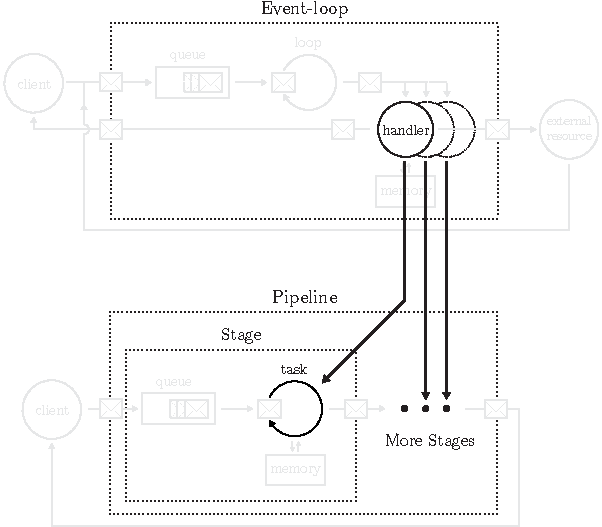
\includegraphics[width=\linewidth]{../resources/run-equivalence.pdf}
    \label{fig:run-equivalence}
    \caption{Equivalence between handlers and tasks}
  \end{minipage}
  \vrule
  \hfill
  \begin{minipage}{0.49\textwidth}
    \centering
    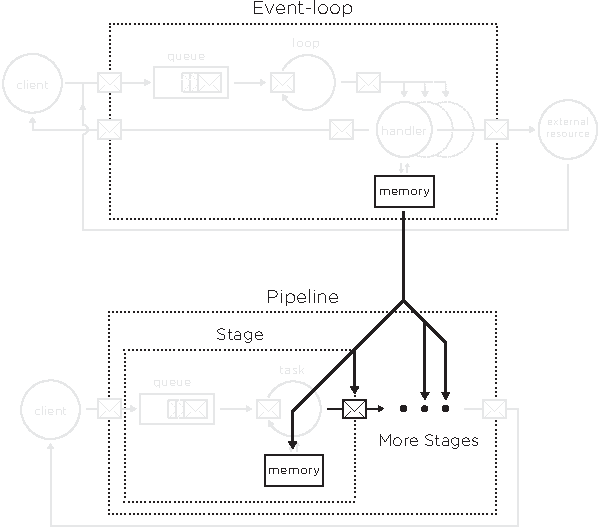
\includegraphics[width=\linewidth]{../resources/mem-equivalence.pdf}
    \label{fig:mem-equivalence}
    \caption{Distribution of the global memory abstraction with message passing}
  \end{minipage}
\end{figure}

\subsection{Continuous Development}

%It proposes this equivalence as a solution to allow the same platform to propose a continuity of compromises between productivity and efficiency.
This equivalence allows a continuity of compromises between productivity and efficiency.
It doesn't intends to enforce both at the same time, but can continuously follow the shift of focus during development.

It allows developers to constantly keep two organizations of their implementation. %, allowing them to start with productivity, and seamlessly abandon it for efficiency as the project matures.
At first, developers start development with the productivity of the multi-paradigms languages, such as Javascript, following the global memory abstraction and the asynchronous control flow of the event-driven execution model.
The focus remains on productivity of development rather than the efficiency of execution.
The application is at least as efficient as with the original event-driven execution model.
Then, during the maturation of the application, the focus continuously shift towards efficiency.
The transformation of the application helps developers to enforce efficiency through continuous iteration to isolate stages.
They can identify the dependencies avoiding parallelism, and arrange the implementation accordingly.

The next paragraphs present the event-driven execution model as the source of this transformation, and the pipeline architecture as the target.